%% bare_conf.tex
%% V1.3
%% 2007/01/11
%% by Michael Shell
%% See:
%% http://www.michaelshell.org/
%% for current contact information.
%%
%% This is a skeleton file demonstrating the use of IEEEtran.cls
%% (requires IEEEtran.cls version 1.7 or later) with an IEEE conference paper.
%%
%% Support sites:
%% http://www.michaelshell.org/tex/ieeetran/
%% http://www.ctan.org/tex-archive/macros/latex/contrib/IEEEtran/
%% and
%% http://www.ieee.org/

%%*************************************************************************
%% Legal Notice:
%% This code is offered as-is without any warranty either expressed or
%% implied; without even the implied warranty of MERCHANTABILITY or
%% FITNESS FOR A PARTICULAR PURPOSE! 
%% User assumes all risk.
%% In no event shall IEEE or any contributor to this code be liable for
%% any damages or losses, including, but not limited to, incidental,
%% consequential, or any other damages, resulting from the use or misuse
%% of any information contained here.
%%
%% All comments are the opinions of their respective authors and are not
%% necessarily endorsed by the IEEE.
%%
%% This work is distributed under the LaTeX Project Public License (LPPL)
%% ( http://www.latex-project.org/ ) version 1.3, and may be freely used,
%% distributed and modified. A copy of the LPPL, version 1.3, is included
%% in the base LaTeX documentation of all distributions of LaTeX released
%% 2003/12/01 or later.
%% Retain all contribution notices and credits.
%% ** Modified files should be clearly indicated as such, including  **
%% ** renaming them and changing author support contact information. **
%%
%% File list of work: IEEEtran.cls, IEEEtran_HOWTO.pdf, bare_adv.tex,
%%                    bare_conf.tex, bare_jrnl.tex, bare_jrnl_compsoc.tex
%%*************************************************************************

% *** Authors should verify (and, if needed, correct) their LaTeX system  ***
% *** with the testflow diagnostic prior to trusting their LaTeX platform ***
% *** with production work. IEEE's font choices can trigger bugs that do  ***
% *** not appear when using other class files.                            ***
% The testflow support page is at:
% http://www.michaelshell.org/tex/testflow/



% Note that the a4paper option is mainly intended so that authors in
% countries using A4 can easily print to A4 and see how their papers will
% look in print - the typesetting of the document will not typically be
% affected with changes in paper size (but the bottom and side margins will).
% Use the testflow package mentioned above to verify correct handling of
% both paper sizes by the user's LaTeX system.
%
% Also note that the "draftcls" or "draftclsnofoot", not "draft", option
% should be used if it is desired that the figures are to be displayed in
% draft mode.
%
\documentclass[10pt, conference, compsocconf]{IEEEtran}
% Add the compsocconf option for Computer Society conferences.
%
% If IEEEtran.cls has not been installed into the LaTeX system files,
% manually specify the path to it like:
% \documentclass[conference]{../sty/IEEEtran}

\usepackage{minted}
\usepackage{mathtools}


% Some very useful LaTeX packages include:
% (uncomment the ones you want to load)


% *** MISC UTILITY PACKAGES ***
%
%\usepackage{ifpdf}
% Heiko Oberdiek's ifpdf.sty is very useful if you need conditional
% compilation based on whether the output is pdf or dvi.
% usage:
% \ifpdf
%   % pdf code
% \else
%   % dvi code
% \fi
% The latest version of ifpdf.sty can be obtained from:
% http://www.ctan.org/tex-archive/macros/latex/contrib/oberdiek/
% Also, note that IEEEtran.cls V1.7 and later provides a builtin
% \ifCLASSINFOpdf conditional that works the same way.
% When switching from latex to pdflatex and vice-versa, the compiler may
% have to be run twice to clear warning/error messages.






% *** CITATION PACKAGES ***
%
%\usepackage{cite}
% cite.sty was written by Donald Arseneau
% V1.6 and later of IEEEtran pre-defines the format of the cite.sty package
% \cite{} output to follow that of IEEE. Loading the cite package will
% result in citation numbers being automatically sorted and properly
% "compressed/ranged". e.g., [1], [9], [2], [7], [5], [6] without using
% cite.sty will become [1], [2], [5]--[7], [9] using cite.sty. cite.sty's
% \cite will automatically add leading space, if needed. Use cite.sty's
% noadjust option (cite.sty V3.8 and later) if you want to turn this off.
% cite.sty is already installed on most LaTeX systems. Be sure and use
% version 4.0 (2003-05-27) and later if using hyperref.sty. cite.sty does
% not currently provide for hyperlinked citations.
% The latest version can be obtained at:
% http://www.ctan.org/tex-archive/macros/latex/contrib/cite/
% The documentation is contained in the cite.sty file itself.






% *** GRAPHICS RELATED PACKAGES ***
%
\ifCLASSINFOpdf
  \usepackage[pdftex]{graphicx}
  % declare the path(s) where your graphic files are
  % \graphicspath{{../pdf/}{../jpeg/}}
  % and their extensions so you won't have to specify these with
  % every instance of \includegraphics
  % \DeclareGraphicsExtensions{.pdf,.jpeg,.png}
\else
  % or other class option (dvipsone, dvipdf, if not using dvips). graphicx
  % will default to the driver specified in the system graphics.cfg if no
  % driver is specified.
  \usepackage[dvips]{graphicx}
  % declare the path(s) where your graphic files are
  % \graphicspath{{../eps/}}
  % and their extensions so you won't have to specify these with
  % every instance of \includegraphics
  % \DeclareGraphicsExtensions{.eps}
\fi
% graphicx was written by David Carlisle and Sebastian Rahtz. It is
% required if you want graphics, photos, etc. graphicx.sty is already
% installed on most LaTeX systems. The latest version and documentation can
% be obtained at: 
% http://www.ctan.org/tex-archive/macros/latex/required/graphics/
% Another good source of documentation is "Using Imported Graphics in
% LaTeX2e" by Keith Reckdahl which can be found as epslatex.ps or
% epslatex.pdf at: http://www.ctan.org/tex-archive/info/
%
% latex, and pdflatex in dvi mode, support graphics in encapsulated
% postscript (.eps) format. pdflatex in pdf mode supports graphics
% in .pdf, .jpeg, .png and .mps (metapost) formats. Users should ensure
% that all non-photo figures use a vector format (.eps, .pdf, .mps) and
% not a bitmapped formats (.jpeg, .png). IEEE frowns on bitmapped formats
% which can result in "jaggedy"/blurry rendering of lines and letters as
% well as large increases in file sizes.
%
% You can find documentation about the pdfTeX application at:
% http://www.tug.org/applications/pdftex





% *** MATH PACKAGES ***
%
%\usepackage[cmex10]{amsmath}
% A popular package from the American Mathematical Society that provides
% many useful and powerful commands for dealing with mathematics. If using
% it, be sure to load this package with the cmex10 option to ensure that
% only type 1 fonts will utilized at all point sizes. Without this option,
% it is possible that some math symbols, particularly those within
% footnotes, will be rendered in bitmap form which will result in a
% document that can not be IEEE Xplore compliant!
%
% Also, note that the amsmath package sets \interdisplaylinepenalty to 10000
% thus preventing page breaks from occurring within multiline equations. Use:
%\interdisplaylinepenalty=2500
% after loading amsmath to restore such page breaks as IEEEtran.cls normally
% does. amsmath.sty is already installed on most LaTeX systems. The latest
% version and documentation can be obtained at:
% http://www.ctan.org/tex-archive/macros/latex/required/amslatex/math/





% *** SPECIALIZED LIST PACKAGES ***
%
\usepackage{algorithmic}
% algorithmic.sty was written by Peter Williams and Rogerio Brito.
% This package provides an algorithmic environment fo describing algorithms.
% You can use the algorithmic environment in-text or within a figure
% environment to provide for a floating algorithm. Do NOT use the algorithm
% floating environment provided by algorithm.sty (by the same authors) or
% algorithm2e.sty (by Christophe Fiorio) as IEEE does not use dedicated
% algorithm float types and packages that provide these will not provide
% correct IEEE style captions. The latest version and documentation of
% algorithmic.sty can be obtained at:
% http://www.ctan.org/tex-archive/macros/latex/contrib/algorithms/
% There is also a support site at:
% http://algorithms.berlios.de/index.html
% Also of interest may be the (relatively newer and more customizable)
% algorithmicx.sty package by Szasz Janos:
% http://www.ctan.org/tex-archive/macros/latex/contrib/algorithmicx/




% *** ALIGNMENT PACKAGES ***
%
%\usepackage{array}
% Frank Mittelbach's and David Carlisle's array.sty patches and improves
% the standard LaTeX2e array and tabular environments to provide better
% appearance and additional user controls. As the default LaTeX2e table
% generation code is lacking to the point of almost being broken with
% respect to the quality of the end results, all users are strongly
% advised to use an enhanced (at the very least that provided by array.sty)
% set of table tools. array.sty is already installed on most systems. The
% latest version and documentation can be obtained at:
% http://www.ctan.org/tex-archive/macros/latex/required/tools/


%\usepackage{mdwmath}
%\usepackage{mdwtab}
% Also highly recommended is Mark Wooding's extremely powerful MDW tools,
% especially mdwmath.sty and mdwtab.sty which are used to format equations
% and tables, respectively. The MDWtools set is already installed on most
% LaTeX systems. The lastest version and documentation is available at:
% http://www.ctan.org/tex-archive/macros/latex/contrib/mdwtools/


% IEEEtran contains the IEEEeqnarray family of commands that can be used to
% generate multiline equations as well as matrices, tables, etc., of high
% quality.


%\usepackage{eqparbox}
% Also of notable interest is Scott Pakin's eqparbox package for creating
% (automatically sized) equal width boxes - aka "natural width parboxes".
% Available at:
% http://www.ctan.org/tex-archive/macros/latex/contrib/eqparbox/





% *** SUBFIGURE PACKAGES ***
%\usepackage[tight,footnotesize]{subfigure}
% subfigure.sty was written by Steven Douglas Cochran. This package makes it
% easy to put subfigures in your figures. e.g., "Figure 1a and 1b". For IEEE
% work, it is a good idea to load it with the tight package option to reduce
% the amount of white space around the subfigures. subfigure.sty is already
% installed on most LaTeX systems. The latest version and documentation can
% be obtained at:
% http://www.ctan.org/tex-archive/obsolete/macros/latex/contrib/subfigure/
% subfigure.sty has been superceeded by subfig.sty.



%\usepackage[caption=false]{caption}
%\usepackage[font=footnotesize]{subfig}
% subfig.sty, also written by Steven Douglas Cochran, is the modern
% replacement for subfigure.sty. However, subfig.sty requires and
% automatically loads Axel Sommerfeldt's caption.sty which will override
% IEEEtran.cls handling of captions and this will result in nonIEEE style
% figure/table captions. To prevent this problem, be sure and preload
% caption.sty with its "caption=false" package option. This is will preserve
% IEEEtran.cls handing of captions. Version 1.3 (2005/06/28) and later 
% (recommended due to many improvements over 1.2) of subfig.sty supports
% the caption=false option directly:
% \usepackage[caption=false,font=footnotesize]{subfig}
%
% The latest version and documentation can be obtained at:
% http://www.ctan.org/tex-archive/macros/latex/contrib/subfig/
% The latest version and documentation of caption.sty can be obtained at:
% http://www.ctan.org/tex-archive/macros/latex/contrib/caption/




% *** FLOAT PACKAGES ***
%
%\usepackage{fixltx2e}
% fixltx2e, the successor to the earlier fix2col.sty, was written by
% Frank Mittelbach and David Carlisle. This package corrects a few problems
% in the LaTeX2e kernel, the most notable of which is that in current
% LaTeX2e releases, the ordering of single and double column floats is not
% guaranteed to be preserved. Thus, an unpatched LaTeX2e can allow a
% single column figure to be placed prior to an earlier double column
% figure. The latest version and documentation can be found at:
% http://www.ctan.org/tex-archive/macros/latex/base/



%\usepackage{stfloats}
% stfloats.sty was written by Sigitas Tolusis. This package gives LaTeX2e
% the ability to do double column floats at the bottom of the page as well
% as the top. (e.g., "\begin{figure*}[!b]" is not normally possible in
% LaTeX2e). It also provides a command:
%\fnbelowfloat
% to enable the placement of footnotes below bottom floats (the standard
% LaTeX2e kernel puts them above bottom floats). This is an invasive package
% which rewrites many portions of the LaTeX2e float routines. It may not work
% with other packages that modify the LaTeX2e float routines. The latest
% version and documentation can be obtained at:
% http://www.ctan.org/tex-archive/macros/latex/contrib/sttools/
% Documentation is contained in the stfloats.sty comments as well as in the
% presfull.pdf file. Do not use the stfloats baselinefloat ability as IEEE
% does not allow \baselineskip to stretch. Authors submitting work to the
% IEEE should note that IEEE rarely uses double column equations and
% that authors should try to avoid such use. Do not be tempted to use the
% cuted.sty or midfloat.sty packages (also by Sigitas Tolusis) as IEEE does
% not format its papers in such ways.





% *** PDF, URL AND HYPERLINK PACKAGES ***
%
%\usepackage{url}
% url.sty was written by Donald Arseneau. It provides better support for
% handling and breaking URLs. url.sty is already installed on most LaTeX
% systems. The latest version can be obtained at:
% http://www.ctan.org/tex-archive/macros/latex/contrib/misc/
% Read the url.sty source comments for usage information. Basically,
% \url{my_url_here}.





% *** Do not adjust lengths that control margins, column widths, etc. ***
% *** Do not use packages that alter fonts (such as pslatex).         ***
% There should be no need to do such things with IEEEtran.cls V1.6 and later.
% (Unless specifically asked to do so by the journal or conference you plan
% to submit to, of course. )

\usepackage{flushend}


% correct bad hyphenation here
\hyphenation{op-tical net-works semi-conduc-tor}


\begin{document}
%
% paper title
% can use linebreaks \\ within to get better formatting as desired
\title{Fast Access to Columnar, Hierarchical Data via Code Transformation}


% author names and affiliations
% use a multiple column layout for up to two different
% affiliations

\author{\IEEEauthorblockN{Jim Pivarski, Peter Elmer}
\IEEEauthorblockA{Physics Department\\
Princeton University\\
Princeton, NJ, 08544\\
pivarski@princeton.edu, peter.elmer@cern.ch}
\and
\IEEEauthorblockN{Brian Bockelman, Zhe Zhang}
\IEEEauthorblockA{Department of Physics and Astronomy\\
University of Nebraska-Lincoln\\
Lincoln, NE 68588\\
bbockelm@cse.unl.edu, zhan0915@huskers.unl.edu}
}

% conference papers do not typically use \thanks and this command
% is locked out in conference mode. If really needed, such as for
% the acknowledgment of grants, issue a \IEEEoverridecommandlockouts
% after \documentclass

% for over three affiliations, or if they all won't fit within the width
% of the page, use this alternative format:
% 
%\author{\IEEEauthorblockN{Michael Shell\IEEEauthorrefmark{1},
%Homer Simpson\IEEEauthorrefmark{2},
%James Kirk\IEEEauthorrefmark{3}, 
%Montgomery Scott\IEEEauthorrefmark{3} and
%Eldon Tyrell\IEEEauthorrefmark{4}}
%\IEEEauthorblockA{\IEEEauthorrefmark{1}School of Electrical and Computer Engineering\\
%Georgia Institute of Technology,
%Atlanta, Georgia 30332--0250\\ Email: see http://www.michaelshell.org/contact.html}
%\IEEEauthorblockA{\IEEEauthorrefmark{2}Twentieth Century Fox, Springfield, USA\\
%Email: homer@thesimpsons.com}
%\IEEEauthorblockA{\IEEEauthorrefmark{3}Starfleet Academy, San Francisco, California 96678-2391\\
%Telephone: (800) 555--1212, Fax: (888) 555--1212}
%\IEEEauthorblockA{\IEEEauthorrefmark{4}Tyrell Inc., 123 Replicant Street, Los Angeles, California 90210--4321}}




% use for special paper notices
%\IEEEspecialpapernotice{(Invited Paper)}




% make the title area
\maketitle


\begin{abstract}
Big Data query systems represent data in a columnar format for fast, selective access, and in some cases (e.g.\ Apache Drill), perform calculations directly on the columnar data without row materialization, avoiding runtime costs.

However, many analysis procedures cannot be easily or efficiently expressed as SQL. In High Energy Physics, the majority of data processing requires nested loops with complex dependencies. When faced with tasks like these, the conventional approach is to convert the columnar data back into an object form, usually with a performance price.

This paper describes a new technique to transform procedural code so that it operates on columnar data natively, without row materialization. It can be viewed as a compiler pass on the typed abstract syntax tree, rewriting references to objects as columnar array lookups.

We will also present performance comparisons between transformed code and conventional object-oriented code in a High Energy Physics context.

\end{abstract}

\begin{IEEEkeywords}
Big data applications; Data structures; Automatic programming; Data analysis; Scientific computing; High energy physics instrumentation computing

\end{IEEEkeywords}


% For peer review papers, you can put extra information on the cover
% page as needed:
% \ifCLASSOPTIONpeerreview
% \begin{center} \bfseries EDICS Category: 3-BBND \end{center}
% \fi
%
% For peerreview papers, this IEEEtran command inserts a page break and
% creates the second title. It will be ignored for other modes.
\IEEEpeerreviewmaketitle



%% \section{Introduction}
%% % no \IEEEPARstart
%% This demo file is intended to serve as a ``starter file''
%% for IEEE conference papers produced under \LaTeX\ using
%% IEEEtran.cls version 1.7 and later.

%% All manuscripts must be in English. These guidelines include complete descriptions of the fonts, spacing, and related information for producing your proceedings manuscripts. Please follow them and if you have any questions, direct them to the production editor in charge of your proceedings at Conference Publishing Services (CPS): Phone +1 (714) 821-8380 or Fax +1 (714) 761-1784.
%% % You must have at least 2 lines in the paragraph with the drop letter
%% % (should never be an issue)

%% \subsection{Subsection Heading Here}
%% Subsection text here.


%% \subsubsection{Subsubsection Heading Here}
%% Subsubsection text here.

%% \section{Type style and Fonts}
%% Wherever Times is specified, Times Roman or Times New Roman may be used. If neither is available on your system, please use the font closest in appearance to Times. Avoid using bit-mapped fonts if possible. True-Type 1 or Open Type fonts are preferred. Please embed symbol fonts, as well, for math, etc.


% An example of a floating figure using the graphicx package.
% Note that \label must occur AFTER (or within) \caption.
% For figures, \caption should occur after the \includegraphics.
% Note that IEEEtran v1.7 and later has special internal code that
% is designed to preserve the operation of \label within \caption
% even when the captionsoff option is in effect. However, because
% of issues like this, it may be the safest practice to put all your
% \label just after \caption rather than within \caption{}.
%
% Reminder: the "draftcls" or "draftclsnofoot", not "draft", class
% option should be used if it is desired that the figures are to be
% displayed while in draft mode.
%
%\begin{figure}[!t]
%\centering
%\includegraphics[width=2.5in]{myfigure}
% where an .eps filename suffix will be assumed under latex, 
% and a .pdf suffix will be assumed for pdflatex; or what has been declared
% via \DeclareGraphicsExtensions.
%\caption{Simulation Results}
%\label{fig_sim}
%\end{figure}

% Note that IEEE typically puts floats only at the top, even when this
% results in a large percentage of a column being occupied by floats.


% An example of a double column floating figure using two subfigures.
% (The subfig.sty package must be loaded for this to work.)
% The subfigure \label commands are set within each subfloat command, the
% \label for the overall figure must come after \caption.
% \hfil must be used as a separator to get equal spacing.
% The subfigure.sty package works much the same way, except \subfigure is
% used instead of \subfloat.
%
%\begin{figure*}[!t]
%\centerline{\subfloat[Case I]\includegraphics[width=2.5in]{subfigcase1}%
%\label{fig_first_case}}
%\hfil
%\subfloat[Case II]{\includegraphics[width=2.5in]{subfigcase2}%
%\label{fig_second_case}}}
%\caption{Simulation results}
%\label{fig_sim}
%\end{figure*}
%
% Note that often IEEE papers with subfigures do not employ subfigure
% captions (using the optional argument to \subfloat), but instead will
% reference/describe all of them (a), (b), etc., within the main caption.


% An example of a floating table. Note that, for IEEE style tables, the 
% \caption command should come BEFORE the table. Table text will default to
% \footnotesize as IEEE normally uses this smaller font for tables.
% The \label must come after \caption as always.
%
%\begin{table}[!t]
%% increase table row spacing, adjust to taste
%\renewcommand{\arraystretch}{1.3}
% if using array.sty, it might be a good idea to tweak the value of
% \extrarowheight as needed to properly center the text within the cells
%\caption{An Example of a Table}
%\label{table_example}
%\centering
%% Some packages, such as MDW tools, offer better commands for making tables
%% than the plain LaTeX2e tabular which is used here.
%\begin{tabular}{|c||c|}
%\hline
%One & Two\\
%\hline
%Three & Four\\
%\hline
%\end{tabular}
%\end{table}


% Note that IEEE does not put floats in the very first column - or typically
% anywhere on the first page for that matter. Also, in-text middle ("here")
% positioning is not used. Most IEEE journals/conferences use top floats
% exclusively. Note that, LaTeX2e, unlike IEEE journals/conferences, places
% footnotes above bottom floats. This can be corrected via the \fnbelowfloat
% command of the stfloats package.



%% \section{Conclusion}
%% The conclusion goes here. this is more of the conclusion

% conference papers do not normally have an appendix


% use section* for acknowledgement
%% \section*{Acknowledgment}


%% The authors would like to thank...
%% more thanks here


% trigger a \newpage just before the given reference
% number - used to balance the columns on the last page
% adjust value as needed - may need to be readjusted if
% the document is modified later
%\IEEEtriggeratref{8}
% The "triggered" command can be changed if desired:
%\IEEEtriggercmd{\enlargethispage{-5in}}

% references section

% can use a bibliography generated by BibTeX as a .bbl file
% BibTeX documentation can be easily obtained at:
% http://www.ctan.org/tex-archive/biblio/bibtex/contrib/doc/
% The IEEEtran BibTeX style support page is at:
% http://www.michaelshell.org/tex/ieeetran/bibtex/
%\bibliographystyle{IEEEtran}
% argument is your BibTeX string definitions and bibliography database(s)
%\bibliography{IEEEabrv,../bib/paper}
%
% <OR> manually copy in the resultant .bbl file
% set second argument of \begin to the number of references
% (used to reserve space for the reference number labels box)

\section{Motivation}

Analysis procedures can be roughly categorized by whether they are easily expressed as transformations of data tables into new tables, by SQL or an SQL variant, rather than a general-purpose programming language. We must emphasize that ``easily expressed'' is subjective, and therefore illustrate with progressively more complex examples.

Suppose we have High Energy Physics (HEP) data in a table with the following schema.

\vspace{0.15 cm}
\begin{minted}{sql}
CREATE TYPE PARTICLE FROM
    STRUCT<pt: DOUBLE,
           eta: DOUBLE,
           phi: DOUBLE>;

CREATE TABLE events (
    eventId INT,
    muons   ARRAY<PARTICLE>,
    jets    ARRAY<PARTICLE>,
    UNIQUE KEY eventId
);
\end{minted}

\vspace{0.15 cm}
\noindent Often the first exploratory action in a HEP analysis is to plot a distribution of the highest particle {\tt pt} {\it per event.} We could do that in SQL by exploding the {\tt muons} into a virtual table and aggregating the maximum {\tt pt}, grouped by {\tt eventId}. If the execution engine loses track of the fact that unique values of {\tt eventId} are contiguous in the exploded table, the query would unnecessarily search the entire dataset for {\tt eventId} matches. A Python or C++ program would not.

The second action a HEP analyst usually takes is to compute masses from {\tt pt}, {\tt eta}, and {\tt phi} of pairs of particles\footnote{$\sqrt{2 {p_1}^{p_T} {p_2}^{p_T} (\cosh({p_1}^\eta - {p_2}^\eta) - \cos({p_1}^\phi - {p_2}^\phi))}$ for $p_1$ and $p_2$}, to see if any were the decay products of a short-lived intermediary. Candidates for such a decay would always be found in the same event, so this query in SQL would involve a full outer join on two exploded {\tt muons} tables or exploded {\tt muons} and exploded {\tt jets}, subject to equal {\tt eventId}. In this case, it is even more important that the uniqueness of {\tt eventId} is tracked, since a join across a distributed database can be very expensive.

HEP data manipulations only get more complex from there. The problem is that the hierarchically nested schema is a poor fit to the relational model for which SQL was designed. Tree-like, nested data are much easier to deal with in a procedural or functional language, particularly one with object-oriented features.

However, sequentially iterating over a large set of objects and applying a user defined function to each can be much slower than a database query, even when parallelized. Databases enjoy several advantages: (1) indexing by primary keys, (2) columnar data layout, and (3) code manipulation (``term rewriting''). Indexing is beyond the scope of this paper, but columnar data layouts are increasingly being used to store hierarchical data. Code manipulation of general purpose programming languages is only common at the compiler level, but data analysis frameworks are beginning to use Just-In-Time (JIT) compilation and metaprogramming in their workflows.

ROOT\cite{root}, the HEP analysis framework, was first to store hierarchical data structures as columns. The ROOT file format (in ``split mode'') stores primitive attributes adjacent to one another on disk, e.g.\ all muon {\tt pt} values, followed by all muon {\tt eta} values, etc. Google independently developed Dremel\cite{dremel}, on which Apache Parquet is based. Spark 2.0 and Apache Arrow extend this concept to data in memory, and each has seen substantial increases in data throughput when switching to a columnar layout, especially for processes that access only a few of the attributes.

JIT compilation is central to machine learning tools like H2O\cite{h2o} and Theano\cite{theano}, Julia\cite{julia}, a scientific programming language, as well as ROOT. To our knowledge, however, none of these manipulate the user's code to match the structure of columnar data.

In this paper, we propose a technique to transform user code to more quickly access columnar data in memory. This technique is inspired by similar methods used on SQL, but SQL tightly controls all loops over data, making the transformation easier. We find that it can be performed on general user code if an Abstract Syntax Tree (AST) with type information is provided, or in conjunction with a type-inference pass over an untyped AST. The user code does not need to walk through the data in order, though it would benefit from fewer cache misses if it is sequential with a regular stride, just like any procedural program.

In fact, code transformation could be viewed as a general alternative to object deserialization: when faced with user code that expects objects but the data are in another form, one could either transform the data to fit the code's expectations (deserialization) or transform the code to fit the data. Deserialization is the more common choice, and the only practical one for complex data formats, but code transformation can be much faster. When manipulating code, the data format is only interpreted once at compile-time. When manipulating data, the format is interpreted once per object, in addition to extra memory allocations and copying.

\section{Data Representation}

We begin by describing the scope of data types we are considering. To simplify the transformations, we restrict this set as much as possible while still being useful. In particular, the data types described here only encode data; they don't determine how data are used, such as which functions can be legally called on them. However, an interpretation layer can be overlaid on this representation without affecting the format or code transformations.

\subsection{Type System}
\label{type-system}

The set of possible types is generated by four constructors:
\begin{itemize}
\item {\bf Primitive:} fixed byte-width booleans, integers, floating point numbers, and possibly characters.
\item {\bf List:} arbitrary-length list of another type, including nested lists.
\item {\bf Union:} represents objects that can be one of several types (``sum types'' in type theory).
\item {\bf Record:} a container mapping field names to types (``product types'' in type theory).
\end{itemize}
We call this type system PLUR, an acronym of the four constructors. A complete type schema in PLUR is a tree of Lists, Unions, and Records whose leaves are Primitive types.

One thing to notice is that this system does not allow for recursively defined types. For instance, one cannot make a ``Tree'' Record containing Trees. All data structures have a finite maximum depth. The pointer mechanism described below makes up for this deficiency.

Another thing to notice is that Records are not named, as structs and classes are in C++. This allows for flexible structural typing, in which the only criteria for a type to be accepted as the argument to a function is that it has the minimum set of fields. If stronger type safety is desired, extra metadata can be added to the type description to indicate type names and/or subclass relationships.

As a concrete example, names can distinguish a raw List$\langle$byte$\rangle$ from a String or even a UTF8String, which should be interpreted in different ways by user code. Similarly, nullable data can be represented as an Option$\langle$X$\rangle$, which is a List$\langle$X$\rangle$ that only allows zero (empty, null) or one (filled) elements.

A particularly useful type is Pointer$\langle$X$\rangle$, which is an integer interpreted as a List index. In addition to having a type name that distinguishes it from ordinary integers, this type would have metadata identifying another List in the structure; dereferencing the pointer returns the item at the List index. With this mechanism, not only can tree data be constructed, but graphs with cycles as well. It also provides a way to compactly represent selected events from large datasets, since a physicist's ``event list'' is a List$\langle$Pointer$\langle$Events$\rangle\rangle$.

\subsection{Objects to Arrays}

Any data described by the PLUR type system can be converted into a set of named arrays. The array names all begin with a user-provided prefix, so that the user can manage arrays representing different objects in a single object store, zip file, HDF5 file, or Python dictionary. Names are generated by a recursive walk over the type structure, and in fact the type schema is losslessly preserved in the names themselves. This may be useful if an external metadata system is not available to store the type schema.

Data are packed into arrays by recursively applying the following rules to a given name $N$ and type $T$ in the structure, where $N = \mbox{the}$ prefix and $T = \mbox{the}$ whole type schema at the root of the data structure.

{\bf If $T$ is a Primitive}, append the primitive value to an array named $N$, creating it if it doesn't yet exist.

{\bf If $T$ is a List} with contained type $T'$ and length $\ell$, find an array named $N + \mbox{``-Lo''}$ (list offset). If it does not yet exist, create it with a single element $0$. Then select the last element $e$ from this array and append $\ell + e$ to the end of the array.

Next, iterate through each item in the List and apply the rule for $T'$ with name $N + \mbox{``-Ld''}$ (list data).

{\bf If $T$ is a Union} with possible types $T_1, \ldots, T_n$ and the datum has actual type $T_t$ (where $t \in [1, n]$), find or create an array named $N + \mbox{``-Ut''}$ (union tag) and append $t$.

Next, follow the rule for name $N + \mbox{``-Ud''} + t$ (union data~$t$) and type $T_t$.

{\bf If $T$ is a Record} with field names and field types $(N_1, T_1), \ldots (N_n, T_n)$, follow the rule for each pair $N_f$, $T_f$ (where $f \in [1, n]$), using $N + \mbox{``-R\_''} + N_f$ (record field $N_f$) as a name and $T_f$ as a type.

A Record does not generate any arrays to represent its structure (as Lists and Unions do); the connection between fields in an array is entirely encoded in the naming convention. To ensure that array names can be properly parsed, field names must not contain the character ``-'' (or a different delimiter should be chosen).

Be sure to include empty/trivial arrays for types that were not touched due to missing data (Lists that are all empty at a given level or Union type possibilities that never occur in the data) or make the reading procedure insensitive to missing arrays. A simple way to include all arrays is to create them with a first pass over the type schema and only append to them in the pass over data.

\subsection{Arrays to Objects}

The procedure described above losslessly stores the type schema in array names and the data in the arrays. To demonstrate this, we describe a procedure for reconstituting objects and types from the arrays and their names.

First, select arrays whose names begin with the prefix and pop the prefix from their names. For each of these arrays $a$, create an index $i_a$ whose initial value is 0. Then recursively apply the following rules.

{\bf If only one array exists and its name is the empty string}, then the type is a Primitive. Take the value at index $i_a$ and increment $i_a$ by~1.

{\bf If one array name begins with ``-Lo'' and all others begin with ``-Ld''}, then the type is a List. Take $a[i_a + 1] - a[i_a]$ as the length $\ell$ of the List and increment $i_a$ by~1 for the array $a$ that begins with ``-Lo''.

Pop the ``-Ld'' from the beginning of all other array names and apply the rule for that set of arrays $\ell$ times.

{\bf If one array name begins with ``-Ut'', and all others begin with ``-Ud''}, then the type is a Union.

Take $a[i_a]$ as the tag $t$ for the datum and increment $i_a$ by~1 for the array $a$ that begins with ``-Ut''.

Pop the $\mbox{``-Ud''} + t$ from the beginning of all other array names associated with tag $t$ and apply the rule for that subset.

{\bf If all array names begin with ``-R\_''}, then the type is a Record. Partition the set of arrays by field name $N_f$, pop the $\mbox{``-R\_''} + N_f$ from the beginning of the array names, and apply the rule separately for each partition to fill each field.

If any other configuration of arrays and names is encountered, the arrays are malformed. If indices go beyond the lengths of the arrays or do not perfectly end on the last element of each array, then the arrays are malformed.

\subsection{Random Access and Redundancy}
\label{random-access-and-redundancy}

The reason that List structures are represented by data offsets (arrays whose names end in ``-Lo''), rather than List lengths, is to permit random access. For instance, if we had a List$\langle$List$\langle$float$\rangle\rangle$ named with prefix ``x'' and we wanted the float at index $(i, j)$, we would compute
\[ \mbox{x-Lo-Ld{\tt [}x-Lo-Lo{\tt [}x-Lo{\tt [}} 0 \mbox{\tt ]} + i \mbox{\tt ]} + j \mbox{\tt ]} \]
At each level, the contents of the ``-Lo'' array are the starting indices of the next-deeper structure.

In fact, if we want to reconstruct only one object in a List, we simply apply the arrays-to-objects algorithm for that List's ``-Ld'' arrays with all indices starting at $i_a = i$.

Random access is a useful feature, but this offset array is not optimal for compression or variable-length integer encoding algorithms. If we wish to store or transmit a List structure in the fewest possible bytes, it should be converted into a corresponding size array (suffix ``-Ls''). For all $i \in [0, \mbox{ length of x-Lo} - 1)$,
\[ \mbox{x-Ls{\tt [}} i \mbox{\tt ]} \coloneqq \mbox{x-Lo{\tt [}} i + 1 \mbox{\tt ]} - \mbox{x-Lo{\tt [}} i \mbox{\tt ]} \]
and vice-versa. (The offset array is one element longer than the size array because we include the initial offset 0, which simplifies the code transformation in the next section.) A nice option would be to transfer or store List structures as size arrays for less redundancy, then expand as offset arrays for random access.

The Union structure, as described so far, is not random accessible. Data arrays for each type possibility $T_t$ are only filled if a datum of that type is observed, so each type possibility must be indexed by a different offset. The arrays-to-objects algorithm described in the previous subsection avoids this issue by walking over the data sequentially.

To make Unions random accessible, we need to add a union offset array ``-Uo''. This can be generated from the tag array ``-Ut'' by
\begin{algorithmic}
\vspace{0.15 cm}
\STATE $i_t \coloneqq 0$ {\bf for all} $t \in [1, n]$

\vspace{0.15 cm}
\FOR{$i \coloneqq 0$ {\bf until} length of x-Ut}
\STATE $t \coloneqq$ \mbox{x-Ut}{\tt [}$i${\tt ]}
\STATE \mbox{x-Uo}{\tt [}$i${\tt ]} $\coloneqq i_t$
\STATE $i_t \coloneqq i_t + 1$
\ENDFOR
\end{algorithmic}

Now we can access Union objects randomly: to reconstruct a Union at index $i$, we find the tag $t$ at x-Ut{\tt [}$i${\tt ]} and follow the arrays-to-objects algorithm on the set of arrays named with the corresponding ``-Ud$t$'', all starting at index $i_t$ given by $\mbox{x-Uo{\tt [}}i\mbox{\tt]}$.

This union offset array is entirely redundant: it can always be generated from a tag array. Therefore, it never needs to be transmitted or stored.

\subsection{Relationship to Apache Arrow}

Readers familiar with Apache Arrow might recognize this object-array encoding\cite{arrow-layout}: it is identical for equivalent Arrow types. Arrow additionally defines null-value masks for each type and headers for seeking to the memory address of each array, rather than assuming a name-based lookup.

With the appropriate translation between PLUR types and Arrow types, array names and Arrow memory addresses, the code transformation procedure described in the next section can be used unmodified on Arrow data, and therefore Pandas\cite{pandas}, R\cite{R}, or SparkSQL\cite{sparksql} DataFrames that are internally represented as Arrow. Alternatively, one could expand our code transformation procedure to cover the Arrow specification natively.

\section{Code Transformation}

An important feature of this data representation is that a structure of any type can be expressed by a single integer, the index that would be used to start the arrays-to-objects algorithm. A type and an array name prefix uniquely specifies a set of arrays, so the only new information at runtime are locations within those arrays.

Only one index is required because:
\begin{itemize}
\item a Primitive value is located at one index in its array;
\item a List's length can be computed from one index \mbox{($a[i_a + 1] - a[i_a]$)} and all of its contents are derived from the value of its offset array at that index;
\item a Union is specified by a tag from its tag array and an offset from its offset array, which occur at the same index. All of the contents are derived from the offset;
\item a Record is just a bundle of fields with no structure array. However, the contents of all fields in one Record start at the same index.
\end{itemize}

Therefore, any function that references Primitive, List, Union, and Record objects, no matter how complicated, can be replaced with a function that references integer indices. We can shape the code to match the data format, rather than shaping the data to match the object-oriented vocabulary of the code.

To see this as an alternative to deserialization, consider a scenario in which all arrays are in a binary file on disk that has been memory-mapped to look like an array. When the transformed code accesses a structured object, it is actually reading values from disk. No additional representation of the data is created; the new function knows what to do from the raw byte values and proceeds as the old function would have with objects. We have skipped deserialization.

The technique described below can be applied to code written in any language, but all of the explicit examples are for Python code because our implementation\cite{plur} transforms Python code.

\subsection{General Strategy}

Unlike SQL, procedural and functional programming languages can assign and possibly reassign variables, extract substructure as new variables, loop over substructure, and pass objects to other functions, where they are identified with new names. It is not sufficient to only transform symbols that coincide with prefix names, since parts of the data structure may be spread among user-defined variables. To avoid missing code that needs to be transformed, we must track the PLUR type of all symbols in the function.

We therefore need a typed AST, in which PLUR types and array name prefixes are associated with any expression nodes that hold non-Primitive PLUR type. (Knowledge of other types is not necessary but not harmful.) The prefixes must be propagated with the type because different parts of a data structure may have the same type but different values, and the correct array references need to be injected into the code. Code transformation and type propagation may be performed in a single sweep.

There are several constraints on the code to be transformed. It cannot create or change PLUR objects, which is reasonable for an analysis procedure. It can use external functions, but if a non-Primitive PLUR object is passed as an argument to such a function, the code for that function must be accessible so that it can be transformed, too. If the same function is called in different places with different PLUR types/names as arguments, multiple versions of the transformed function will be generated. These external functions cannot be created or passed dynamically; their code must be accessible for conversion during the transformation sweep.

The following AST nodes must be transformed:
\begin{itemize}
\item {\bf symbol reference}, which might be a PLUR object;
\item {\bf assignment}, which might pass PLUR type and prefix to a new symbol;
\item {\bf list subscript} (square brackets in most languages), which can dereference a PLUR List;
\item {\bf attribute subscript} (dot in most languages), which can dereference a PLUR Record;
\item {\bf function calls}, which can pass PLUR types and prefixes to a new function, widening the scope of the transformation sweep to include that function, and may return a PLUR type/prefix that must be tracked;
\item {\bf special functions}, like {\tt len} (List length) and {\tt isinstance} (check type) in Python, which have to be handled in special ways when called on PLUR types.
\end{itemize}

Any use of a PLUR type that isn't specially handled must be treated as an error to avoid misinterpretations. Since this transformation sweep is performed on an AST, often before the transformed code is further transformed by a low-level compiler, these errors would appear to the user as compilation errors, preferably with line numbers and meaningful error messages.

\subsection{Required Transformations}

{\bf Symbol references} are leaves of the AST and therefore first to be transformed in the recursive walk. In the original function, an identifier that refers to a PLUR object becomes an identifier for its integer index, so a symbol reference becomes array extraction.

For Primitive and List types:
\begin{center}
{\tt x} (referring to object) $\to$ {\tt array[x]} ({\tt x} is index)
\end{center}
where {\tt array} is the only array associated with a Primitive and the list offset associated with a List.

Unions immediately resolve to their specific type (unless you require the user to ``unpack'' opaque Union objects with a function). This is most easily handled by (1) creating a new symbol in the transformed code to hold the tag value and (2) checking each tag possibility, returning the offset of the appropriate one:
\begin{center}
{\tt x} $\to$ {\tt t $\coloneqq$ tag[x]; if (t == 0) off[x] \ldots}
\end{center}
This is more difficult in languages like Python, which do not allow assignment in an expression (the symbol reference can appear anywhere in an expresssion); see our Python implementation\cite{plur} for the work-around.

References to Record symbols do not require any transformation at all, though they are reinterpreted as indices to be passed to fields.

{\bf Assignment} merely passes the PLUR type and associated array names to a new symbol. In the type-inference pass, this means adding the type information to a symbol table.

Assignment is more complex if you try to handle pattern matching, such as Python's tuple unpacking (see ``Flourishes'' below).

{\bf List subscripts} replace a List index with a Primitive value if it is a List of Primitives or the index of the next substructure down if it is any other type. This can be performed in two steps: (1) transform
\begin{center}
{\tt x[i]} $\to$ {\tt off[x + i]}
\end{center}
and then (2) transform the result of this as though it were a symbol reference (rule described above) using the List's item type.

An attempt to subscript any PLUR type other than a List is an error. The above only works if the index resolves to integer type, not (for example) a Python {\tt slice}. Handling slices would be considered a flourish.

{\bf Attribute subscripts} extract a field from a Record by name. In most languages, the field names are syntactically required to be a string known at compile-time with constraints on the characters (usually, ``-'' is not allowed).

We do this transformation in two steps, like the list subscript above: (1) transform
\begin{center}
{\tt x.fieldname} $\to$ {\tt x}
\end{center}
and then (2) transform the result of this as though it were a symbol reference (rule described above) using the selected field type.

An attempt to subscript any PLUR type other than a Record is an error.

{\bf Function calls} can either include non-Primitive PLUR types in their arguments or not. If a function call does not reference any non-Primitive PLUR types, it can be left as-is (after transforming the arguments).

If it references non-PLUR types, then we must obtain the AST for that function and propagate PLUR types through it, starting with the argument types. If the function has previously been transformed, then the transformed copy may be reused only if the argument types (and array prefixes) are the same as before. We are treating all functions as though they were type-parameterized in every argument because different array prefixes require different code transformations.

If a function is recursive, then this process will only terminate if previous transformations of the function are saved and reused for the same type arguments. It is not merely an optimization to reuse transformed functions!

A function may return PLUR type; the transformed version is either a Primitive or an integer index that must be propagated from the point of the function call in the original code.

{\bf Special functions} that return meaningful data about non-Primitive PLUR types must be handled on a case-by-case basis. As with any function call, if a non-Primitive PLUR type is an argument, the function's identity must be known during the transformation sweep. Below are two important cases.

{\bf len}: (get length of List) must return the length when given a PLUR List, which is computed as
\begin{center}
{\tt len(x)} $\to$ {\tt off[x + 1] - off[x]}
\end{center}
(applied without transforming the argument {\tt x}, or by reverse-engineering an applied transformation).

{\bf isinstance}: (check type) must return true if the argument has a given type, false otherwise. Since references to non-Primitive PLUR types have all been replaced with integer indices, a naive application of the {\tt isinstance} function would yield true for integers, contrary to a user's expectation.

The type or types to check must be known as literal names, not computed references, during the transformation sweep. If the argument to check has List or Record type, the whole expression should be replaced with true or false depending on whether the desired types are in the set of types to check. If it is a Union, it must be replaced with a tag check.

\subsection{Flourishes}

Depending on your needs, you can provide more or less support for PLUR objects in the transformed code. The only invariant is that the transformed code must either work exactly as object-oriented code would or fail to be transformed (compilation error).

\subsubsection{List Overflows}

One special case requires special attention: what to do about List index overflows? In the minimal transformation described above, PLUR List overflows behave like C array overflows, in that they return undefined results. The errors are less obvious and therefore more dangerous than typical C array overflows because PLUR values just beyond a List's boundary belong to the same attribute in the next List, so they probably have the right scale and distribution, subtly biasing analysis results.

A simple way to eliminate mistakes like this is to add a range check to the transformed code. Indices that fail the range check should raise a runtime exception. It would be correct, but many of these range checks would be unnecessary and would slow down processing. For instance, the list subscript could be in the body of an {\tt if} statement where the user did range-checking manually, or it could be in a {\tt for} loop bounded by the list length (a very common case), or it could be a {\tt foreach} node (Python {\tt for}) that has been transformed from objects to indices (another flourish).

Since we are performing type-inference anyway, we could track intervals of validity for expressions that appear in list subscripts. This is known as a dependent type check, and for our case the validity endpoints should be symbolic: literal integers or $\ell_T$ symbols for the length of List type/array prefix $T$. The symbolic algebra includes only inequality operators, addition and subtraction, logical operators, and restrictions in {\tt if}-{\tt else} blocks. If the expression in a list subscript is not provably between 0 (inclusive) and $\ell_T$ (exclusive), a compilation error tells the user about the possibility of List overflows and refuses to transform the code.

\subsubsection{Pythonic Indices}

Negative index handling in Python would be another flourish, which only slightly complicates the above.

\subsubsection{Fixed-size Arrays and Matrices}

PLUR Lists can have any length, which includes a constant length, at the expense of having redundant offset arrays. The size array for a fixed-length List is filled with identical values, which is very compressible, but must be expanded to full length for random access.

It would be possible to add the concept of a fixed-length List to the type system, along with a naming convention so that this type can be encoded in array names, rather than arrays. In place of an array lookup in the transformed code, one would insert a literal multiplcation.

\subsubsection{Eliminating Zero-Lookups}

As an optimization, one can statically identify array lookups that always return zero: the first element of every list offset array is zero, and the outermost list offset array is always evaluated at its first element. Without explicitly removing it, this unnecessary code would be executed at every step in an iteration over a List. (PLUR-unaware compilers cannot remove it.)

\subsubsection{Type Constructors}

As stated above, passing a non-Primitive PLUR object to any unrecognized function is a compilation error. This especially includes constructors for dynamic objects like Python lists and dictionaries, since we cannot statically track where they are used. However, you may wish to allow some immutable objects to include PLUR objects, such as Python tuples to use Python tuple-unpacking in assignments. You then become obliged, however, to track these objects as containing PLUR types.

\subsubsection{Pattern Matching}

More generally than Python's tuple-unpacking, your target language may feature pattern-matching, and you may need to track PLUR types through syntactical structures like these.

\subsubsection{Equality and Order}

PLUR objects have a natural definition for value-based equality, so you may want to support the {\tt ==} operator as a recursive object comparison. Reference-based equality (``{\tt is}'' in Python) is even easier: just verify that the indices are equal (in Python, replace ``{\tt ==}'' with ``{\tt is}'').

For identical types, there may be a natural ordering as well: Python defines an ordering on structures like Lists and Records. You can similarly support inequality operators and the ``{\tt sorted}'' function.

\subsubsection{Fallback to Object Materialization}

One way to support particularly difficult cases, such as external functions without code transformation, is by materializing objects using the arrays-to-objects algorithm. This gives up on zero-copy efficiency, but it may be worthwhile to mix fast code with expressive code. Then, rather than new features allowing specific cases of user code to run at all, new features would allow the user code to run faster.

\subsubsection{Runtime Types}

As described in Section~\ref{type-system}, basic types described only in terms of Primitive, List, Union, and Record generators should be augmented by higher-level interpretations of these types, distinctions that are relevant for runtime behavior, not data packing. These runtime types would be implemented at this level.

For instance, a String or UTF8String type would be admissible to functions that {\tt capitalize} and {\tt lower}, but List$\langle$byte$\rangle$ would not. The former would be implemented as a special function, like {\tt len} and {\tt isinstance}. Pointers should either be transparently dereferenced (can cause infinite loops) or opaquely with a special function or syntax.

\section{Implementation}

We are developing PLUR and code transformation tools\cite{plur} for use in a HEP query system\cite{hepquery}. The code is in an early but usable state as documented by the text on the GitHub READMEs.

Both are Python projects, and the code transformation implemented in the PLUR package is written in Python, transforming Python code. The short-term goal is to build a query system that uses Python as its query language, with a long term goal of developing a declarative query language on top of PLUR.

\subsection{Pythonic PLUR}

All of the ``required transformations'' (described above) have been implemented except for function calls and the {\tt isinstance} special function. Of the ``flourishes,'' zero-lookups have been eliminated and tuple-unpacking assignments has been implemented. The problem of implementing Union symbol references has been solved by passing nested closures through the transformation sweep.

This PLUR package optionally passes the transformed code to Numba\cite{numba} for an even greater speedup. Although Numba's conversion of Python code to native bytecode results in a much larger speedup factor than PLUR's transformation step alone, the Numba step wouldn't be possible without the PLUR step. The PLUR transformation replaces opaque Python objects with integers and array lookups, which fit squarely in Numba's vocabulary.

\subsection{Columnar Data from ROOT}

The ROOT file format is the universal standard for HEP. Fortunately for our application, ROOT can store hierarchical data in a columnar fashion, smoothing the transition to PLUR. Most of these arrays can be imported without modification. The one exception is that Lists are represented in ROOT with size arrays, rather than offset arrays, so we apply the transformation described in Section~\ref{random-access-and-redundancy}.

ROOT is a C++ framework providing an object-oriented interface, so we also had to bypass part of its deserialization procedure to get the raw arrays directly into PLUR. In a fork of the ROOT project\cite{bulkio}, we added methods to {\tt TBranch} (ROOT's data column) to extract arrays after decompression but before object materialization, as well as methods to expose these as Numpy arrays in Python. These enhancements, known as BulkIO, are being merged into the main ROOT repository with the intention of being included in ROOT version 6.12.

\subsection{Performance Studies}

The goal of this and the HEPQuery project is to make HEP analysis easier to develop and faster to run. We believe that broad type abstractions like PLUR and concise syntax like Python's are easier for data analysts to work with, especially when they are exploring a dataset and focusing on physics and statistics issues, rather than programming. We also intend to make the system as fast as or faster than idiomatic, object-oriented C++, so that analysts don't have to translate analysis code from a high-level language to a low-level one just to process a large dataset in a reasonable time. This is the allure of databases: SQL is as abstract as set theory and yet it is also faster than most procedural code.

For this reason, we have been performance-testing PLUR all through its development, to avoid introducing performance gaffes at an early stage, and now perform an even-handed performance comparison between transformed PLUR code and industry-standard C++ in ROOT. We also break down the differences as much as possible to show where they come from.

We consider four sample analysis functions, two of which (``max p$_{\mbox{\scriptsize T}}$'' and ``mass of pairs'') are from the motivation of this paper. Listings are given in Figure~\ref{four-functions}.

\begin{figure}
\scriptsize

\noindent\begin{minipage}{\textwidth}
\begin{minipage}[c][1.8cm][t]{0.22\linewidth}
\underline{{\bf max p$_{\mbox{\tiny T}}$} in Python}
\begin{minted}{python}
maximum = 0.0
for muon in event.Muon:
  if muon.pt > maximum:
    maximum = muon.pt
fill_histogram(maximum)
\end{minted}
\end{minipage}
\begin{minipage}[c][1.8cm][t]{0.25\linewidth}
\underline{{\bf max p$_{\mbox{\tiny T}}$} in C++}
\begin{minted}{c++}
float maximum = 0.0;
for (i=0; i < muons.size(); i++)
  if (muons[i]->pt > maximum)
    maximum = muons[i]->pt;
fill_histogram(maximum);
\end{minted}
\end{minipage}

\vspace{0.25 cm}
\begin{minipage}[c][2.6cm][t]{0.22\linewidth}
\underline{{\bf eta of best by p$_{\mbox{\tiny T}}$} in Python}
\begin{minted}{python}
maximum = 0.0
best = -1
for muon in event.muons:
  if muon.pt > maximum:
    maximum = muon.pt
    best = muon
if best != -1:
  fill_histogram(maximum)
\end{minted}
\end{minipage}
\begin{minipage}[c][2.6cm][t]{0.25\linewidth}
\underline{{\bf eta of best by p$_{\mbox{\tiny T}}$} in C++}
\begin{minted}{c++}
float maximum = 0.0;
Muon* best = nullptr;
for (i=0; i < muons.size(); i++)
  if (muons[i]->pt > maximum) {
    maximum = muons[i]->pt;
    best = muon; }
if (best != nullptr)
  fill_histogram(best->eta);
\end{minted}
\end{minipage}%

\vspace{0.25 cm}
\begin{minipage}[c][3.2cm][t]{0.22\linewidth}
\underline{{\bf mass of pairs} in Python}
\begin{minted}{python}
n = len(event.muons)
for i in range(n):
  for j in range(i+1, n):
    m1 = event.muons[i]
    m2 = event.muons[j]
    mass = sqrt(
      2*m1.pt*m2.pt*(
      cosh(m1.eta - m2.eta) -
      cos(m1.phi - m2.phi)))
    fill_histogram(mass)
\end{minted}
\end{minipage}
\begin{minipage}[c][3.2cm][t]{0.25\linewidth}
\underline{{\bf mass of pairs} in C++}
\begin{minted}{c++}
int n = muons.size();
for (i=0; i < n; i++)
  for (j=i+1; j < n; j++) {
    Muon* m1 = muons[i];
    Muon* m2 = muons[j];
    double mass = sqrt(
      2*m1->pt*m2->pt*(
      cosh(m1->eta - m2->eta) -
      cos(m1->phi - m2->phi)));
    fill_histogram(mass); }
\end{minted}
\end{minipage}%

\vspace{0.25 cm}
\begin{minipage}[c][2.4cm][t]{0.22\linewidth}
\underline{{\bf p$_{\mbox{\tiny T}}$ sum of pairs} in Python}
\begin{minted}{python}
n = len(event.muons)
for i in range(n):
  for j in range(i+1, n):
    m1 = event.muons[i]
    m2 = event.muons[j]
    s = m1.pt + m2.pt
    fill_histogram(s)
\end{minted}
\end{minipage}
\begin{minipage}[c][2.4cm][t]{0.25\linewidth}
\underline{{\bf p$_{\mbox{\tiny T}}$ sum of pairs} in C++}
\begin{minted}{c++}
int n = muons.size();
for (i=0; i < n; i++)
  for (j=i+1; j < n; j++) {
    Muon* m1 = muons[i];
    Muon* m2 = muons[j];
    double s = m1->pt + m2->pt;
    fill_histogram(s); }
\end{minted}
\end{minipage}%
\end{minipage}

\caption{\label{four-functions} Sample analysis functions in Python (before code transformation) and object-oriented C++, showing only the body of the loop over events.}
\end{figure}

The first, ``max p$_{\mbox{\scriptsize T}}$,'' is an example of a query that would be difficult but not impossible in SQL. Instead of exploding a muons table and grouping by a unique {\tt eventId}, we keep a running maximum that resets in each event.

The second, ``eta of best by p$_{\mbox{\scriptsize T}}$,'' is an extension of that idea: we select a muon by maximizing {\tt pt} and then plot its {\tt eta}. This is even more awkward in SQL, but very common in HEP.

In the listing, note that {\tt best}, which is a muon object, is initialized as $-1$ in Python and {\tt nullptr} in C++. The current implementation of the code transformer is missing a concept of ``undefined variable.'' It is also missing a thorough check on pre-transformation data types, so it doesn't complain about a variable being $-1$ in some cases and a Record object in others. Post-transformation, it is an array index, so $-1$ is allowed and doesn't correspond to any real objects. This is a leaky abstraction and will be corrected in future versions, but convenient for performance testing now.

The third function, ``mass of pairs,'' would require a full outer join in SQL but is a nested for loop in Python and C++, carefully indexed to avoid duplication. This kind of loop is such a common case that a HEP toolbox ought to have a built-in generator for it. The formula for {\tt mass} is complex, but it is one of the most common calculations in HEP.

The fourth, ``p$_{\mbox{\scriptsize T}}$ sum of pairs,'' is a diagnostic of the third. As we will show below, the mass calculation is the slowest of the sample functions, and it was unclear whether the nested indexing was responsible or the complex formula. This function has the same nesting structure but a simpler formula (which is occasionally useful in HEP).

We ran each analysis function on a 5.4 million event dataset of simulated Drell-Yan collisions (a realistic physics sample, one of about a dozen that might be involved in a real HEP analysis). The tests were performed on an {\tt i2.xlarge} instance on Amazon Web Services, which features a large, fast SSD (hundreds of MB/second, not a bottleneck in our tests).

Both tests, Python and C++, used ROOT to read the same data files. However, the Python test used the BulkIO feature to extract and decompress columnar array data without constructing event objects. The C++ code used the conventional interface, which further deserializes the columnar arrays as C++ objects.

One thing that ROOT's conventional interface does not do (but in general a framework might) is allocate memory for the event and muon objects during the event loop. Memory allocation recognized as a performance killer early in ROOT's development, so ROOT's default is to preallocate a buffer of 1000 muons and overwrite them at the start of each event, reallocating the buffer if necessary. (This never happened in our sample; the maximum number of muons was 36, which is far above the mean of 1--2.)

Also, to avoid decompression or physical access being a dominant contributor to all tests, we prepared an uncompressed sample and loaded it into Linux page cache with vmtouch\cite{vmtouch}. This lets us see the differences due to other factors more clearly.

Both tests were single-threaded and had plenty of working space memory.

The results of the study are shown in Figure~\ref{root-and-plur}. The shorthand ``ROOT'' signifies a conventional ROOT workflow, using C++ user code, and ``PLUR'' is our workflow using the BulkIO interface in ROOT to expose columnar data as arrays and then run code-transformed Python code on those arrays.

\begin{figure}[!t]
\centering
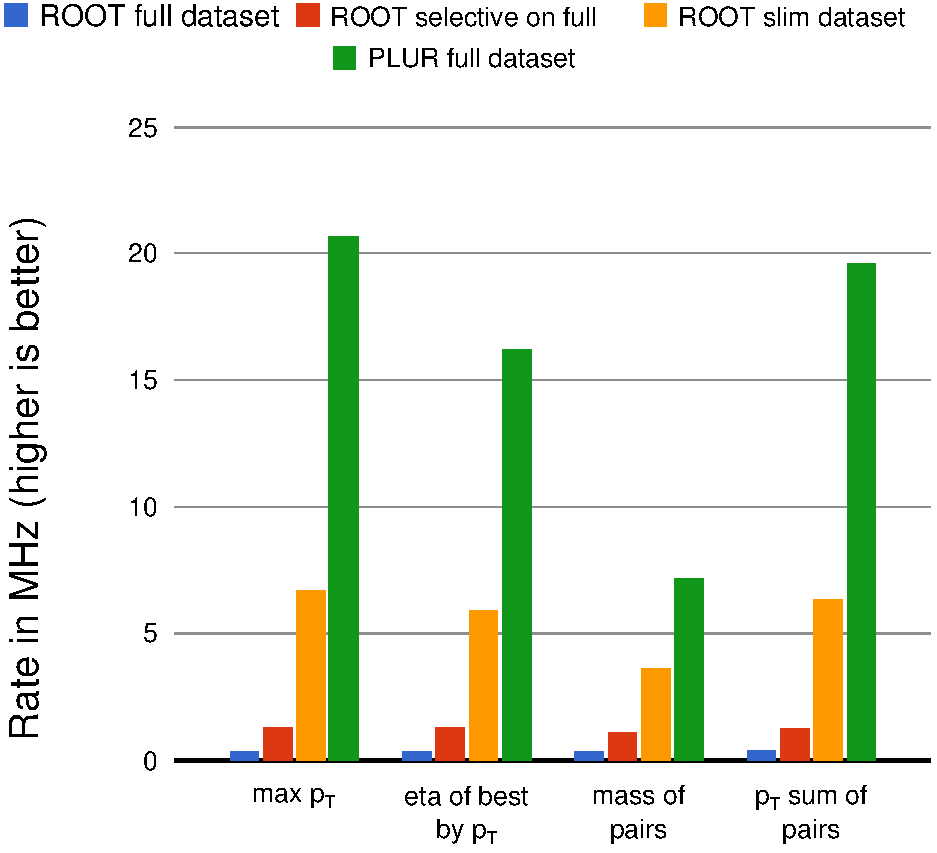
\includegraphics[width=\linewidth]{root-and-plur.pdf}
\caption{Event processing rates, including read and execute times, for 5.4 million events in the test sample. Grouped bars indicate different analysis functions and colors indicate different workflows. See the text for details.}
\label{root-and-plur}
\end{figure}

The four colors signify variants on these workflows. ``ROOT full dataset'' means we let ROOT fill all 42 attributes of the Muon objects, which is clearly unnecessary for our functions. The event processing rate for this case is 0.4~MHz, regardless of the content of the function. Reading and filling the objects overwhelms all other factors.

``ROOT selective on full'' uses ROOT's built-in mechanism to avoid filling all attributes in the objects, but still used the 42-field object definitions and original data file. The event processing rate is 1.29~MHz, regardless of the function. Handling all of the attributes still dominates.

``ROOT slim dataset'' performs the same selective read on a specially prepared dataset and object definition that has only 3 fields: {\tt pt}, {\tt eta}, and {\tt phi}. We now see different rates for the four functions: 6.68, 5.96, 3.56, and 6.34~MHz.

``PLUR full dataset'' is the only test in this batch that uses transformed Python code. It accesses the full dataset (slim dataset yields similar results) and is unaffected by deserialization because the transformed function recognizes the relevant parts of the data arrays on the fly. The four functions are processed at 17.9, 12.1, 6.09, and 17.2~MHz, respectively, considerably faster than the C++.

The slowest of the four functions is ``mass of pairs.'' Unlike the first two functions, this involves a doubly nested loop over muons to find distinct pairs, as well as a much more complex formula. The fourth function has the same structure without the complex formula, and it is as fast as the single loops. Upon further investigation, we found that the trigonometric and hyperbolic cosines account for the majority of the time spent in this function.

The factor that the ROOT tests and PLUR test had in common is that they both extracted data from ROOT files and used part of the ROOT framework to read them. PLUR can operate on any arrays, so we performed another test in which we extracted all the data as Numpy arrays and read them from SSD disk or memory into the transformed Python code. These results are presented in Figure~\ref{physical-media} as ``raw SSD disk'' and ``raw memory.'' The ``PLUR full dataset'' measurements are redrawn in this plot to clarify the change in scale.

\begin{figure}[!t]
\centering
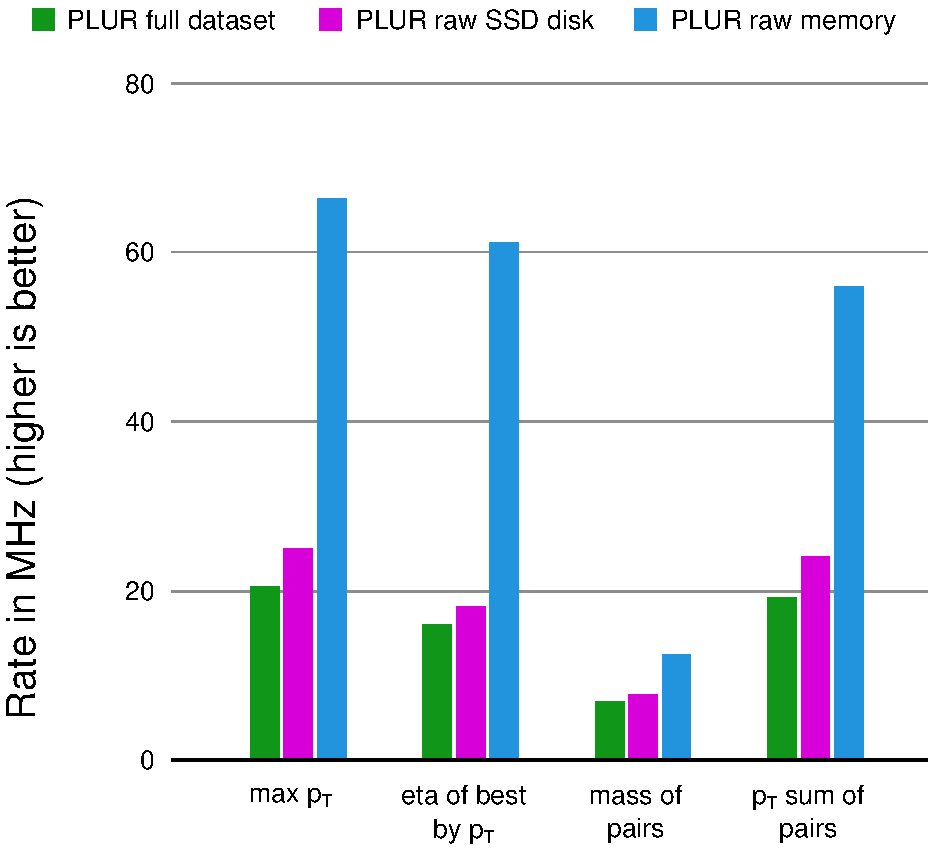
\includegraphics[width=\linewidth]{physical-media.pdf}
\caption{Event processing rates for the same four analysis functions, but only for PLUR workflows. Colors represent data sources: full ROOT dataset, raw Numpy files on SSD disk, and Numpy arrays in memory.}
\label{physical-media}
\end{figure}

When the data are in memory, we see only the calculation cost with no I/O. The effect of the slow mass calculation is dramatic: ``mass of pairs'' runs at 12.8~MHz while ``p$_{\mbox{\scriptsize T}}$ sum of pairs'' runs at 56.2~MHz. Reading from this SSD disk and performing the calculation is 1.6--3.3 times slower than just performing the calculation.

This is relevant because the HEPQuery system is being designed with a two-layer cache: frequently accessed columns will stay in memory, less frequently accessed columns will be paged to an SSD disk like this one, and infrequent or first-time requests will be extracted from ROOT files using BulkIO.

\section{Conclusions}

We have demonstrated that it is possible to transform code to meet a data format, rather than deserializing data to fit the code's expectations, as long as JIT compilation is available. We have also demonstrated that, once transformed and compiled, a Python analysis function outperforms the same function written in idiomatic C++.

On the surface, this is almost unthinkable--- C++ is supposed to be much faster than an abstract language like Python--- that's why HEP data analysts go to great effort to port their Pythonic explorations into C++. However, our code transformation and Numba's bytecode compilation have eliminated Python's disadvantages and given it an advantage not shared by the idiomatic C++, skipping object deserialization. Procedural code is one step closer to behaving like a database query.

In HEP, we plan to use this tool as part of a database-like query server, delivering analysis results in response to queries written in Python. The PLUR data representation gives us the ability to represent large Lists of HEP events, possibly with deeply nested hierarchies and pointer cross-references, as well as random access non-event data used to process these events. Possible uses include lookup tables, calibration constants, boosted decision trees and neural nets.

The use of columns for data granularity, rather than files that contain columns, opens up possibilities for better efficiency in data storage. It is fairly common for a HEP dataset to undergo several revisions, in which derived quantities are progressively corrected with new knowledge. Currently, each new version requires as much disk space as the previous one, which is wasteful if only a few attributes change. With column granularity, a new dataset can be defined using some new and some old columns, like structural sharing in immutable data structures or version control systems like git. Additionally, analysts would be more free to experiment with different event selections if each is just a single column that points to a shared set of publicly accessible events, rather than a copy of a subset of rows.

But perhaps most importantly, the usefulness of this technique is not limited to HEP. The need for complex loop dependencies can hardly be HEP-specific. Although many industries and fields of academia are currently using SQL or languages similar to SQL for data analysis, how much is being left unexplored because the tools are not suited for the task?

It is our wish that this technique finds application in many different fields, just as the techniques of database-style analysis have inspired our work in HEP.

\section*{Acknowledgment}

This material is based upon work supported by the National Science Foundation under Grant No.\ 1450377 and 1450323.

\bibliographystyle{IEEEtran}
\bibliography{IEEEabrv,mybibliography}

\end{document}
